\documentclass[final,hyperref={pdfpagelabels=false}]{beamer}
\mode<presentation>{\usetheme{HugonPoster}}

\usepackage[orientation=portrait,size=a0,scale=1.4,debug]{beamerposter}
\listfiles

\newcommand{\jra}{\ensuremath{\rightarrow}}
\newcommand{\fb}{\,fb$^{-1}$}
\newcommand{\mmm}{\ensuremath{\,\mathrm{M(\mu\mu)}}}
\newcommand{\mjj}{\ensuremath{m_{jj}}}
\newcommand{\deta}{\ensuremath{|\Delta\eta|}}
\newcommand{\pt}{\ensuremath{p_T}}
\newcommand{\ptmm}{\ensuremath{\pt(\mu\mu)}}
\newcommand{\ptmiss}{\ensuremath{\pt^{Miss}}}
\newcommand{\hmm}{\ensuremath{\mathrm{H} \rightarrow \mu^+\mu^-}}
\newcommand{\gghmm}{\ensuremath{gg \rightarrow \hmm{}}}
\newcommand{\vbfhmm}{\ensuremath{\,\mathrm{VBF }\,\hmm{}}}
%\newcommand{\GeVc}{\ensuremath{\,\mathrm{Ge\kern -0.1em V\!/c}}}
%\newcommand{\GeVcc}{\ensuremath{\,\mathrm{Ge\kern -0.1em V\!/c}^2}}
\newcommand{\GeVc}{\,\text{Ge\kern -0.1em V\!/c}}
\newcommand{\GeVcc}{\,\text{Ge\kern -0.1em  V\!/c}\ensuremath{\mathrm{^2}}}
\newcommand{\ttbar}{\ensuremath{t\bar{t}}}
\newcommand{\cls}{CL$\mathrm{_s}$}

%%%%%%%%%%%%%%%%%%%%%%%%%%%%%%%%%%%%%%%%%%%%%%%%%%%%%%%%%%%%%%%%%%%%%%%%%%%%%%%%%%%%%%
 
\title{39) Search for \hmm}
\author{Justin Hugon}
\institute{On Behalf of the CMS Collaboration}
\date{\today}
\email{justin.hugon@cern.ch}

%%%%%%%%%%%%%%%%%%%%%%%%%%%%%%%%%%%%%%%%%%%%%%%%%%%%%%%%%%%%%%%%%%%%%%%%%%%%%%%%%%%%%%
% Must manually figure out what the column height should be.  105cm works well for A0
\newlength{\columnheight}
\setlength{\columnheight}{105.5cm} % for A0

%%%%%%%%%%%%%%%%%%%%%%%%%%%%%%%%%%%%%%%%%%%%%%%%%%%%%%%%%%%%%%%%%%%%%%%%%%%%%%%%%%%%%%
\begin{document}
\begin{frame}
  \begin{columns}
    % ---------------------------------------------------------%
    % Set up a column 
    \begin{column}{.49\textwidth}
      \begin{beamercolorbox}[center,wd=\textwidth]{postercolumn}
        \begin{minipage}[T]{.95\textwidth}  % tweaks the width, makes a new \textwidth
          \parbox[t][\columnheight]{\textwidth}{ % must be some better way to set the the height, width and textwidth simultaneously
            % Since all columns are the same length, it is all nice and tidy.  You have to get the height empirically
            % ---------------------------------------------------------%
            % fill each column with content            
            \begin{block}{\boldmath Why Search for \hmm{}?}
              \begin{itemize}
                \item Smallest Coupling Directly Observable at LHC
                \begin{center}
                  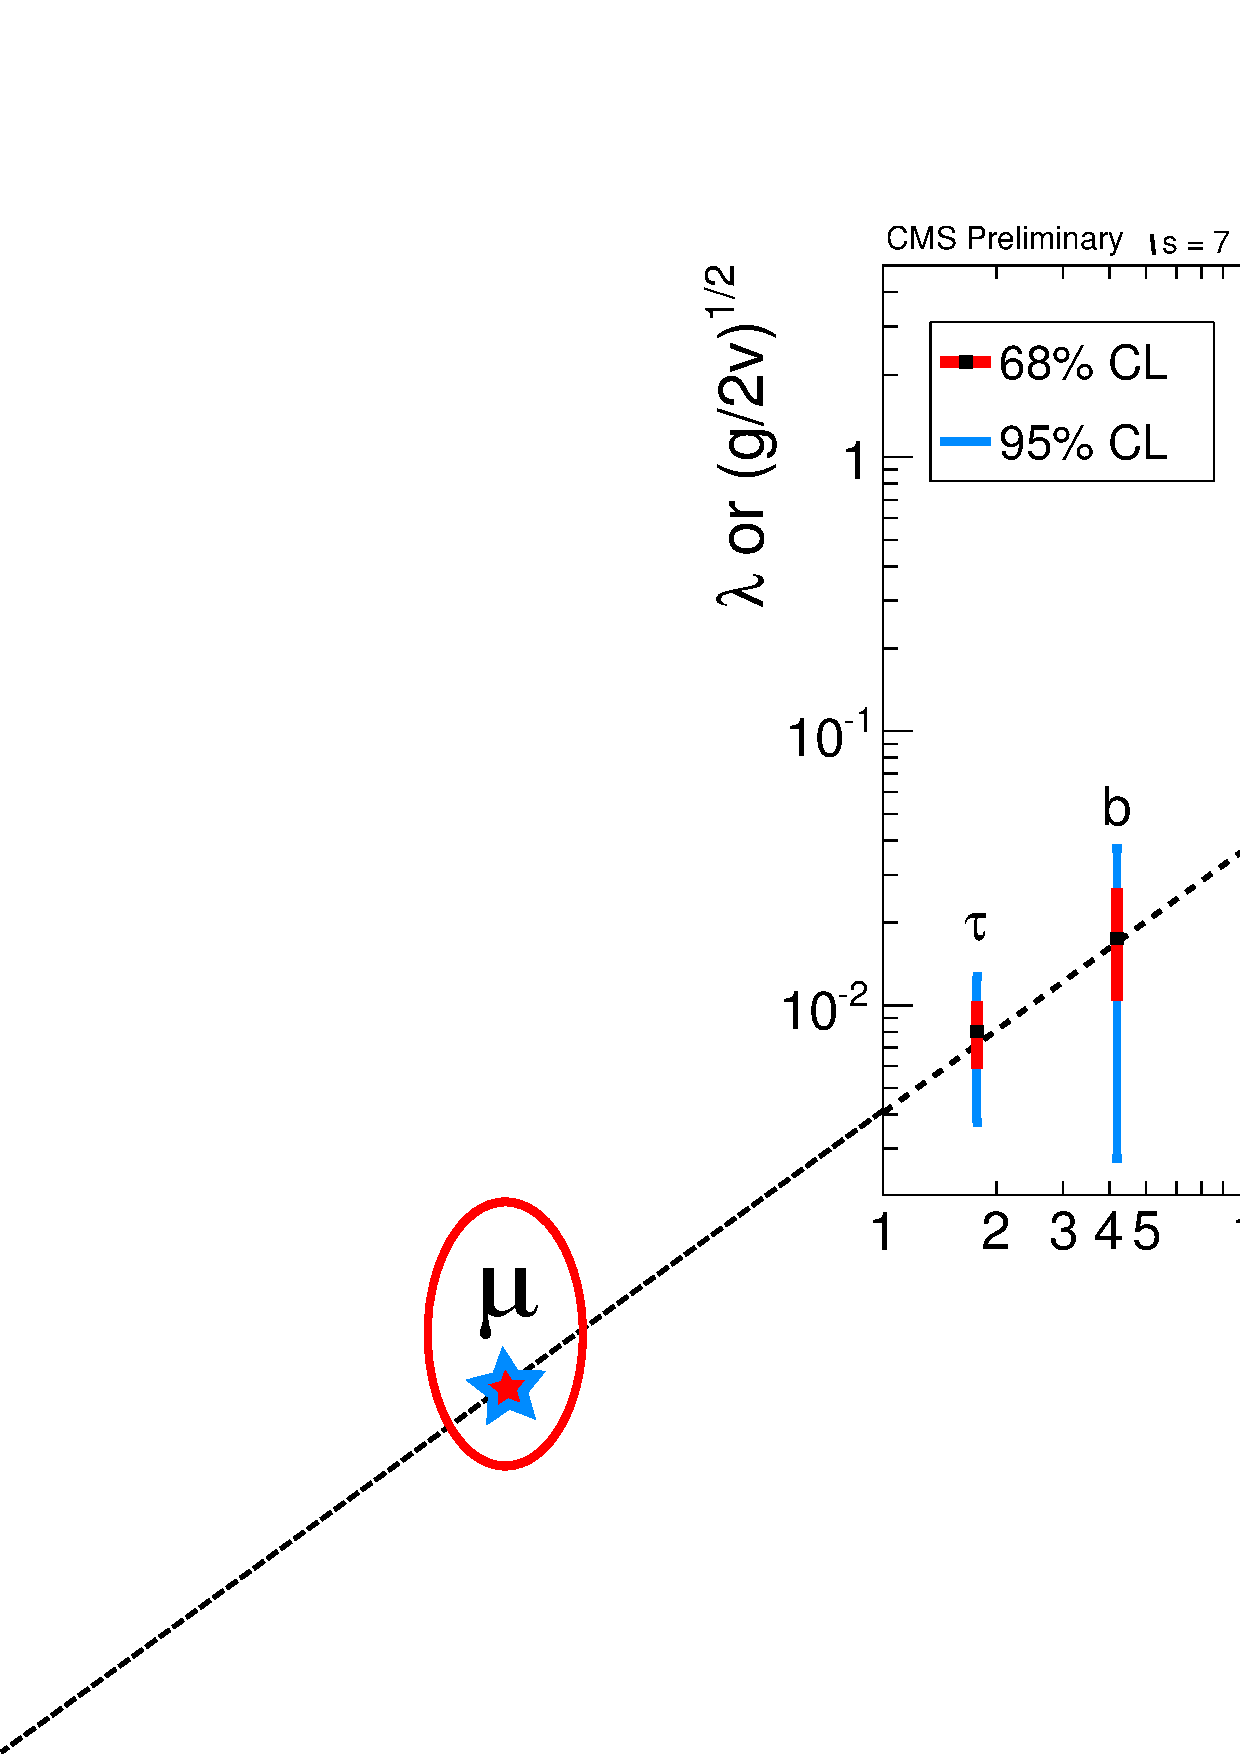
\includegraphics[width=0.55\textwidth]{other/myCouplingVMass3.pdf}
                \end{center}              
                \item Probe 2nd Generation Fermion Coupling
                \item Precisely Predicted in SM
                \item Enhanced in Some New Physics Models
                \item Very Clean Final State
                \begin{itemize}
                  \item Narrow Peak on Smoothly Falling Background
                \end{itemize}              
              \end{itemize}
            \end{block}
            \vfill
            \begin{block}{Search Overview}
              \begin{itemize}
                \item Analyze CMS Data:
                \begin{itemize}
                  \item $5.0 \pm 0.1$ \fb at 7 TeV from 2011
                  \item $19.7 \pm 0.5$ \fb at 8 TeV from 2012
                \end{itemize}              
                \item Trigger on Single Isolated Muon: $\pt>24\GeVc{}$, $|\eta|<2.1$
                \item Require 2 Opposite Sign, Isolated Muons
                \begin{itemize}
                  \item $\pt>25\GeVc{}$, $|\eta|<2.1$
                \end{itemize}              
                \item Divide Events into 2 Categories:
                \begin{itemize}
                  \item 0 or 1 Jet:  Large Acceptance for Gluon Fusion (GF) Higgs Production
                  \item 2 Jet:  Larger S/B for Vector Boson Fusion (VBF) Higgs Production
                \end{itemize}              
                \item Further Sub-categorize to Increase Sensitivity
                \item Perform Shape Fit in Each Subcategory
                \begin{itemize}
                  \item Signal Yield \& Shape Estimated from Simulation Corrected to Match Data
                  \item Background Yield \& Shape Estimated from Fit to Data
                \end{itemize}              
              \end{itemize}
            \end{block}
            \vfill
            \begin{block}{0,1-Jet Subcategories}
              \begin{itemize}
                \item First, Split by \ptmm{}
                \begin{itemize}
                  \item 0,1-Jet Tight: $\ptmm{}\geq10\GeVc{}$
                  \item 0,1-Jet Loose: $\ptmm{}<10\GeVc{}$
                  \item Reduced Drell-Yan Background in 0,1-Jet Tight
                \end{itemize}
                \item Sub-categorize by Muon $|\eta|$, Which is Related to \mmm{} Resolution
                \begin{itemize}
%                  \item Barrel: $|\eta|<0.8$
%                  \item Overlap: $0.8<|\eta|<1.6$
%                  \item Endcap $1.6<|\eta|<2.1$
                  \item Central Dimuons Have Better Mass Resolution
                  \item Signal Peak FWHM at $m_H=125\GeVcc{}$: 3.8-5.9\GeVcc{} 
                \end{itemize}
              \end{itemize}
%              \begin{center}
%                \includegraphics[width=0.50\textwidth]{plotsPublic/controlPlots_analysisA/pdf/nonVBFPresel_dimuonMass_8TeV.pdf}
%                %\\ Background Drell-Yan Dominated
%                \includegraphics[width=0.50\textwidth]{plotsPublic/controlPlots_analysisA/pdf/nonVBFPresel_dimuonPt_8TeV.pdf}
%                %\\ GF Higgs Peaks at Higher \ptmm{}
%              \end{center}
            \end{block}
            \vfill
            \begin{block}{2-Jet Subcategories}
              \begin{itemize}
                \item VBF Higgs Production Mode Enhanced in 2-Jet Category
                \item VBF Tight Sub-Category: 
                \begin{itemize}
                  \item M(jj)$>650\GeVcc{}$ 
                  \item $|\Delta\eta(\mathrm{jj})|>3.5$
                \end{itemize}
                \item GF Tight Sub-Category: 
                \begin{itemize}
                  \item M(jj)$>250\GeVcc{}$ 
                  \item $\ptmm>50\GeVcc{}$
                \end{itemize}
                \item Loose: All Remaining Events
              \end{itemize}
              \begin{center}
                \includegraphics[width=0.45\textwidth]{plotsPublic/controlPlots_analysisA/pdf/dijetMass_8TeV.pdf}
                \includegraphics[width=0.45\textwidth]{plotsPublic/controlPlots_analysisA/pdf/deltaEtaJets_8TeV.pdf}
              \end{center}
            \end{block}
          }
        \end{minipage}
      \end{beamercolorbox}
    \end{column}
    % ---------------------------------------------------------%
    % end the column

    % ---------------------------------------------------------%
    % Set up a column 
    \begin{column}{.49\textwidth}
      \begin{beamercolorbox}[center,wd=\textwidth]{postercolumn}
        \begin{minipage}[T]{.95\textwidth} % tweaks the width, makes a new \textwidth
          \parbox[t][\columnheight]{\textwidth}{ % must be some better way to set the the height, width and textwidth simultaneously
            % Since all columns are the same length, it is all nice and tidy.  You have to get the height empirically
            % ---------------------------------------------------------%
            % fill each column with content
            \begin{block}{Dimuon Mass Distributions}
              \begin{center}
                \includegraphics[width=0.5\textwidth]{plotsPublic/mass_AnanlysisA/pdf/CombSplitAll_8TeV_125_Jets01PassPtG10BB.pdf}
                %\includegraphics[width=0.5\textwidth]{plotsPublic/mass_AnanlysisA/pdf/CombSplitAll_8TeV_125_Jets01PassPtG10BO.pdf}
                %\\
                \includegraphics[width=0.5\textwidth]{plotsPublic/mass_AnanlysisA/pdf/CombSplitAll_8TeV_125_Jet2CutsVBFPass.pdf}
                %\includegraphics[width=0.5\textwidth]{plotsPublic/mass_AnanlysisA/pdf/CombSplitAll_8TeV_125_Jet2CutsGFPass.pdf}
              \\
              Signal PDF: Gaussian + Gaussian; Background PDF: $\frac{\exp(p_1 m_{\mu\mu})}{(m_{\mu\mu}-p_2)^2}$
              \end{center}
            \end{block}
            \vfill
            \begin{block}{Results}
              \begin{itemize}
                \item 95\% \cls Upper Limits for $m_H = 125 \GeVcc{}$:
                \begin{itemize}
                  \item Expected Limit: $5.1^{+2.3}_{-1.5}\times$SM
                  \item Observed Limit: $7.4\times$SM
                \end{itemize}              
                \item Best Fit $\sigma/\sigma_{\mathrm{SM}}=2.9^{+2.8}_{-2.7}$ for CMS Higgs Mass Estimate 125.7\GeVcc{} (CMS-PAS-HIG-13-005)
              \end{itemize}              
              \begin{center}
                \includegraphics[width=0.5\textwidth]{plotsPublic/limits_annalysisA/pdf/CombSplitAll_7P8TeV.pdf}
                \includegraphics[width=0.5\textwidth]{plotsPublic/pValues_analysisA/pdf/pValues_Final7P8TeV.pdf}
              \end{center}
              \begin{itemize}
                \item $1\sigma$ Excess Observed Near 125\GeVcc{}
                \item Maximum Local Significance: $2.3\sigma$
                \item Global Significance: $0.8\sigma$
                \item No Significant Excess Found
              \end{itemize}
            \end{block}
            \vfill
            \begin{block}{\boldmath Projections to $\mathbf{\sqrt{s}=14}$ TeV -- arXiv:1307.7135 }
               \begin{itemize} 
                  \item Method:
                  \begin{itemize} 
                    \item Use 8 TeV Analysis \& Samples 
                    \item Rescale Cross-Sections to $\sqrt{s}=14$ TeV
                  \end{itemize}
                  \item Systematics Scenarios:
                  \begin{itemize}
                    \item Scenario 1: All Uncertainties Same as Current Analysis
                    \item Scenario 2: Experimental Uncertainties Scale $1/\sqrt{\mathcal{L}}$, \\
                                      Theoretical Uncertainties Cut in Half
                  \end{itemize}
                  \item Exclude SM with $175^{+150}_{-75}$\fb
               \end{itemize}
               \begin{center}
                      \begin{tabular}{|l|c|c|} \hline
                          & 300\fb & 3000\fb \\ \hline
                        Significance  & $2.5\sigma$ & $7.9\sigma$ \\ \hline
                        Error on $\sigma/\sigma_{SM}$ Scenario 1  & 42\% & 20\% \\ \hline
                        Error on $\sigma/\sigma_{SM}$ Scenario 2  & 40\% & 14\% \\ \hline
                        Error on Muon Coupling Scenario 1  & 23\% & 8\% \\ \hline
                        Error on Muon Coupling Scenario 2  & 23\% & 7.5\% \\ \hline
                      \end{tabular}
               \end{center}
            \end{block}
            \vfill
            \begin{block}{Conclusions}
              \begin{itemize}
                \item Search Performed for Higgs Decays to $\mu^+\mu^-$
                %\begin{itemize}
                %  \item Interesting Decay Mode Sensitive to New Physics
                %\end{itemize}
                \item Increase Sensitivity by Categorizing Events According to 
                        Production Mode, \ptmm{}, Muon $|\eta|$, and Di-jet Variables
                \item Most Significant Excess Found $\sim1\sigma$
                \item 95\% \cls{} Limit on $\sigma/\sigma_{SM}$ for $m_H= 125\GeVcc{}$:
                \begin{itemize}
                  \item Expected: $5.1^{+2.3}_{-1.5}\times$SM
                  \item Observed: $7.4\times$SM
                \end{itemize}
                \item Best Fit $\sigma/\sigma_{SM}=2.9^{+2.8}_{-2.7}$ for $m_H= 125.7\GeVcc{}$
              \end{itemize}
            \end{block}
          }
          % ---------------------------------------------------------%
          % end the column
        \end{minipage}
      \end{beamercolorbox}
    \end{column}
    % ---------------------------------------------------------%
    % end the column
  \end{columns}
  \vskip1ex
  \tiny\hfill{Created with \LaTeX \texttt{beamerposter}  \url{http://www-i6.informatik.rwth-aachen.de/~dreuw/latexbeamerposter.php} \hskip1em}
\end{frame}
\end{document}
